\section{Bluetooth LE/Smart}
	\begin{tabular}{ll}
		\parbox{10cm}{
			\begin{itemize}
				\item Brand new protocol stack compared to BR/EDR
				\item Target: Ultra low power application which runs with coin cell battery
				\item Works with 40 channels of 2 MHz in the 2.4 GHz band
				\item GFSK Modulation (Gaussian Frequency Shift Keying)
				\item Bitrate of 1 Mb/s
				\item client server architecture
				\item Only star networks possible
				\item Uses advertising events on 3 channels to broadcast data without established connection (no hopping, using 3 channels in sequence)
				\item Data exchange with frequency hopping on 37 data channels when connection established
			\end{itemize}

		}	
		& \parbox{8cm}{
			\fbox{ 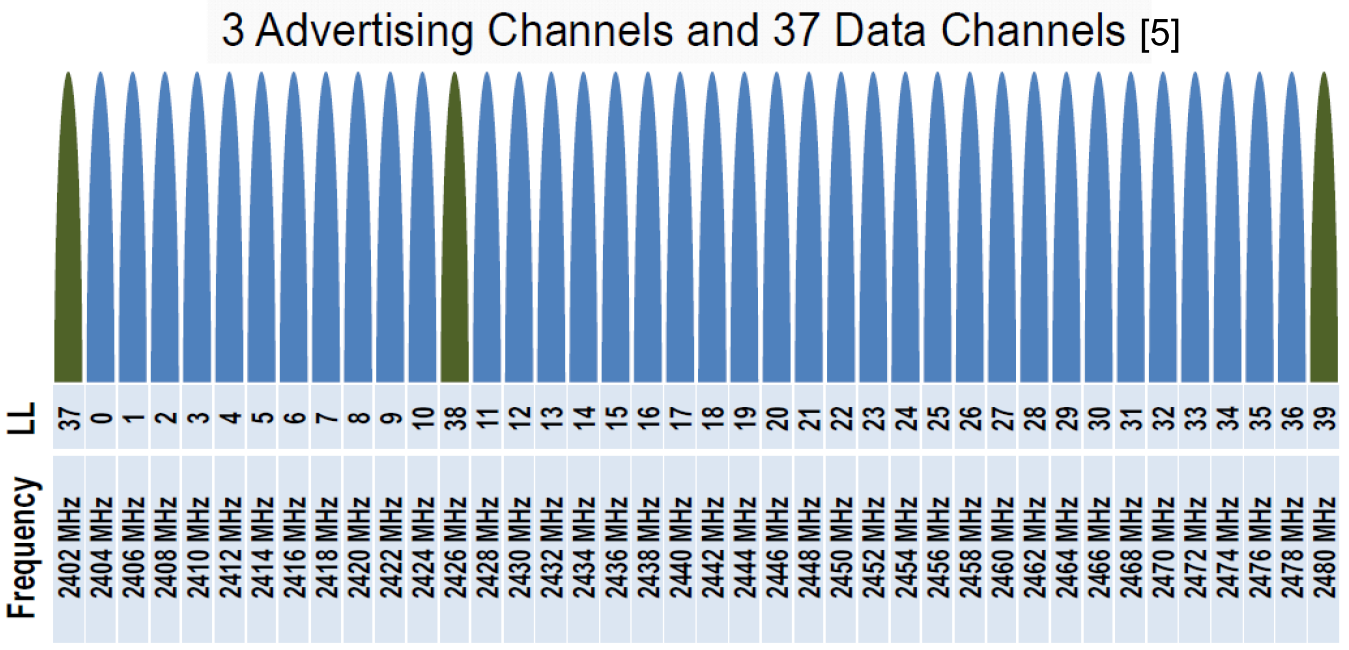
\includegraphics[width=8cm]{./bilder/ble-channels.png}} \\ BLE advertising and data channels }
	\end{tabular}
	
	\subsection{Topology}
		\begin{tabular}{ll}
			\parbox{9cm}{
				\fbox{ 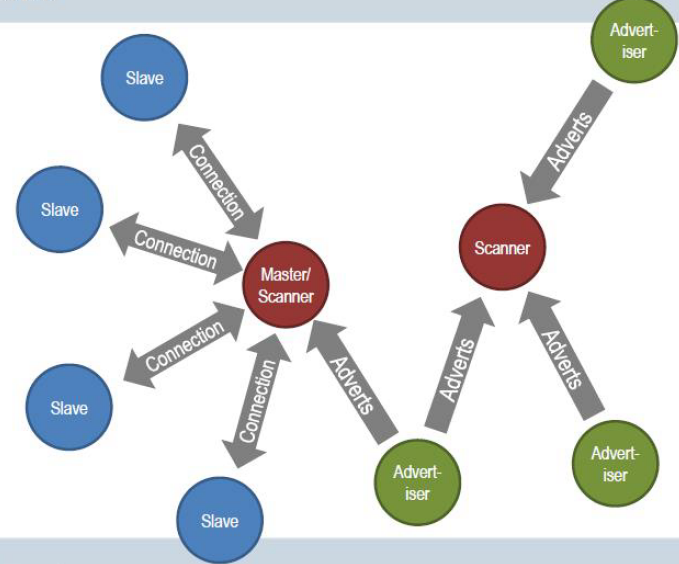
\includegraphics[width=8cm]{./bilder/ble-topology.png}} \\ BLE Topology 
			}	
			& \parbox{9cm}{
				Maximum 4 slaves are available at the moment on the market. However, the BLE standard doesn't define a maximum number of slaves.
				
				Compared to BT-BR/EDR the master is communicating on different frequencies with the slaves.
				With BLE it is not possible to have scatternet anymore.
			}	
		\end{tabular}
